\documentclass[10pt]{article}
\usepackage[czech]{babel}
\usepackage{graphicx}
\usepackage{tabulary}
\usepackage{href-ul}
\usepackage{listings}
\usepackage{color}

\graphicspath{{./images/.}}

\author{Ondřej Nedojedlý\thanks{SPŠ elektrotechnická, Makarenkova 1; Mgr. Tomáš Michalek}}
\date{25. Listopadu, 2023}
\title{\Huge{\bf{Stopky}}}

\begin{document}

\maketitle

\tableofcontents
\listoffigures
\listoftables

\newpage

\section{Zadání}

Vytvoření programu na přípravku \textbf{STM32F407VGT6U} s \textbf{RTOS-RTX4}, jež bude fungovat jako jednoduché stopky.
Porgram bude zobrazovat na prvním řádku LCD čas, který začně běžet od začátku programu.
Čas bude ve formátu:

$$MM:SS:mmm$$

kde:  
\begin{itemize}
\item[\textbf{M}] jsou minuty,
\item[\textbf{S}] jsou sekundy,
\item[\textbf{m}] jsou millisekundy.
\end{itemize}

Po zmáčknutí uživatelského tlačítka, se na druhý řádek LCD dispeje zobrazí čas v okamžiku
zmáčknutí tlačítka. Nová časová stopa se nahraje až při opětovném zmáčknutí uživatelského talačítka;
při držení se nenahrává stále nová časová stopa.

\section{Teoretický rozbor}

Pro pochopení běhu programu, jeho funkcionality a možných problému je nutno míti solidní základy
teoriteckého rázu, jinak bude zpracováni úlohy problematické.

\subsection{Popis přípravku}

Jak avizováno výše, jedná se o přípravek STM32F407VTG6U od firmy STMicroelectronics. Přípravek
je 32-bitový Arm® Cortex®-M4 architektury RISC, přípravek je zaobalen ve
STM32F4-DISCOVERY kitu (Obrázek \ref{fig:kit}).

\begin{figure}[h]
    \centering
    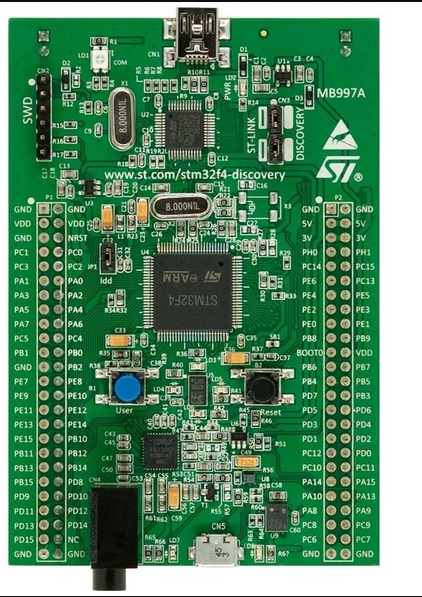
\includegraphics[scale=0.3]{kit.png}
    \caption{STM32F4 discovery kit}
    \label{fig:kit}
\end{figure}

\newpage

STM32F4xx podporuje:
\begin{itemize}
    \item Analogový generátor náhodných čísel,
    \item 15 komunikačních sběrnic,
    \item Dva 12-bitové DA převodníky,
    \item Tři 12-bitové AD převodníky,
    \item 17 časovačů,
    \item 1-MB flash paměti,
    \item 132-KB RAM paměti,
    \item ST-LINK, pro nahrávání programů,
    \item \ldots 
    
\end{itemize}

Jedná periferie, kterou je nutno připojit jest LCD.

\subsubsection{LCD}

Připojení LCD k STM32F4-Discovery je provedeno přes piny dle tabulky \ref{tab:lcdstm}.
Jedná se konkrétně LCD 1602A verze 1.3.


\begin{table}[!htb]
    \begin{minipage}{0.45\textwidth}
        \centering
        \begin{tabular}{c|c}
            LCD & STM32F4 \\
            \hline \\
            RS & PE3 \\
            RW & PE4 \\
            E  & PE5 \\ 
            D4 & PE6 \\
            D5 & PE7 \\
            D6 & PE8 \\
            D7 & PE9
        \end{tabular}
        
        \caption{Připojení LCD k STM32F4 Discovery}
        \label{tab:lcdstm}
    \end{minipage}
    \hfil
    \begin{minipage}{0.45\textwidth}
        \centering
        \begin{tabular}{c|c}
            LCD & připojení \\
            \hline \\
            VSS & GND \\
            VDD & +5v \\
            D0  & NC  \\
            D1  & NC  \\
            D2  & NC  \\
            D3  & NC  \\
            A   & +5v \\
            K   & +5v \\
            V0  & Napěťový dělič
        \end{tabular}
        \caption{Připojení dalších pinů LCD}
        \label{tab:lcdother}
    \end{minipage}
\end{table}

Pro funkčnost LCD je nutno ještě zapojit piny dle tabulky \ref{tab:lcdother},
jinak nebude nice zobrazeno. 

\subsection{Popis softwaru}

Vývoj je činěn v µVision IDE. Jako knihovny použijeme:

\begin{itemize}
    \item [\href{https://www.github.com/spsehavirov/stm32kit}{\textbf{stm32\_kit}}] Knihovna nám umožní provést abstrakci nad CMIS;

    \item [\textbf{RTX4}] Vytvoření RTOS, namísto superloopy;
\end{itemize}

\subsubsection{RTOS}

\textbf{R}eal-\textbf{T}ime \textbf{O}perační \textbf{S}ystém je druh operačních systému který nám umožňuje práci s kriticky náročnými požadavky,
jelokož u GPOS není zaručeně dáno (kromě IRS), že se činnost provede do času $k$. RTOS definuje tasky\footnote{Někdy je "task" chápán jako synonymum ke slovu "thread".}, které jsou zaměňovány dle R-R algoritmu.

\subsection{Vývojový diagram}

\begin{figure}[h]
    \centering
    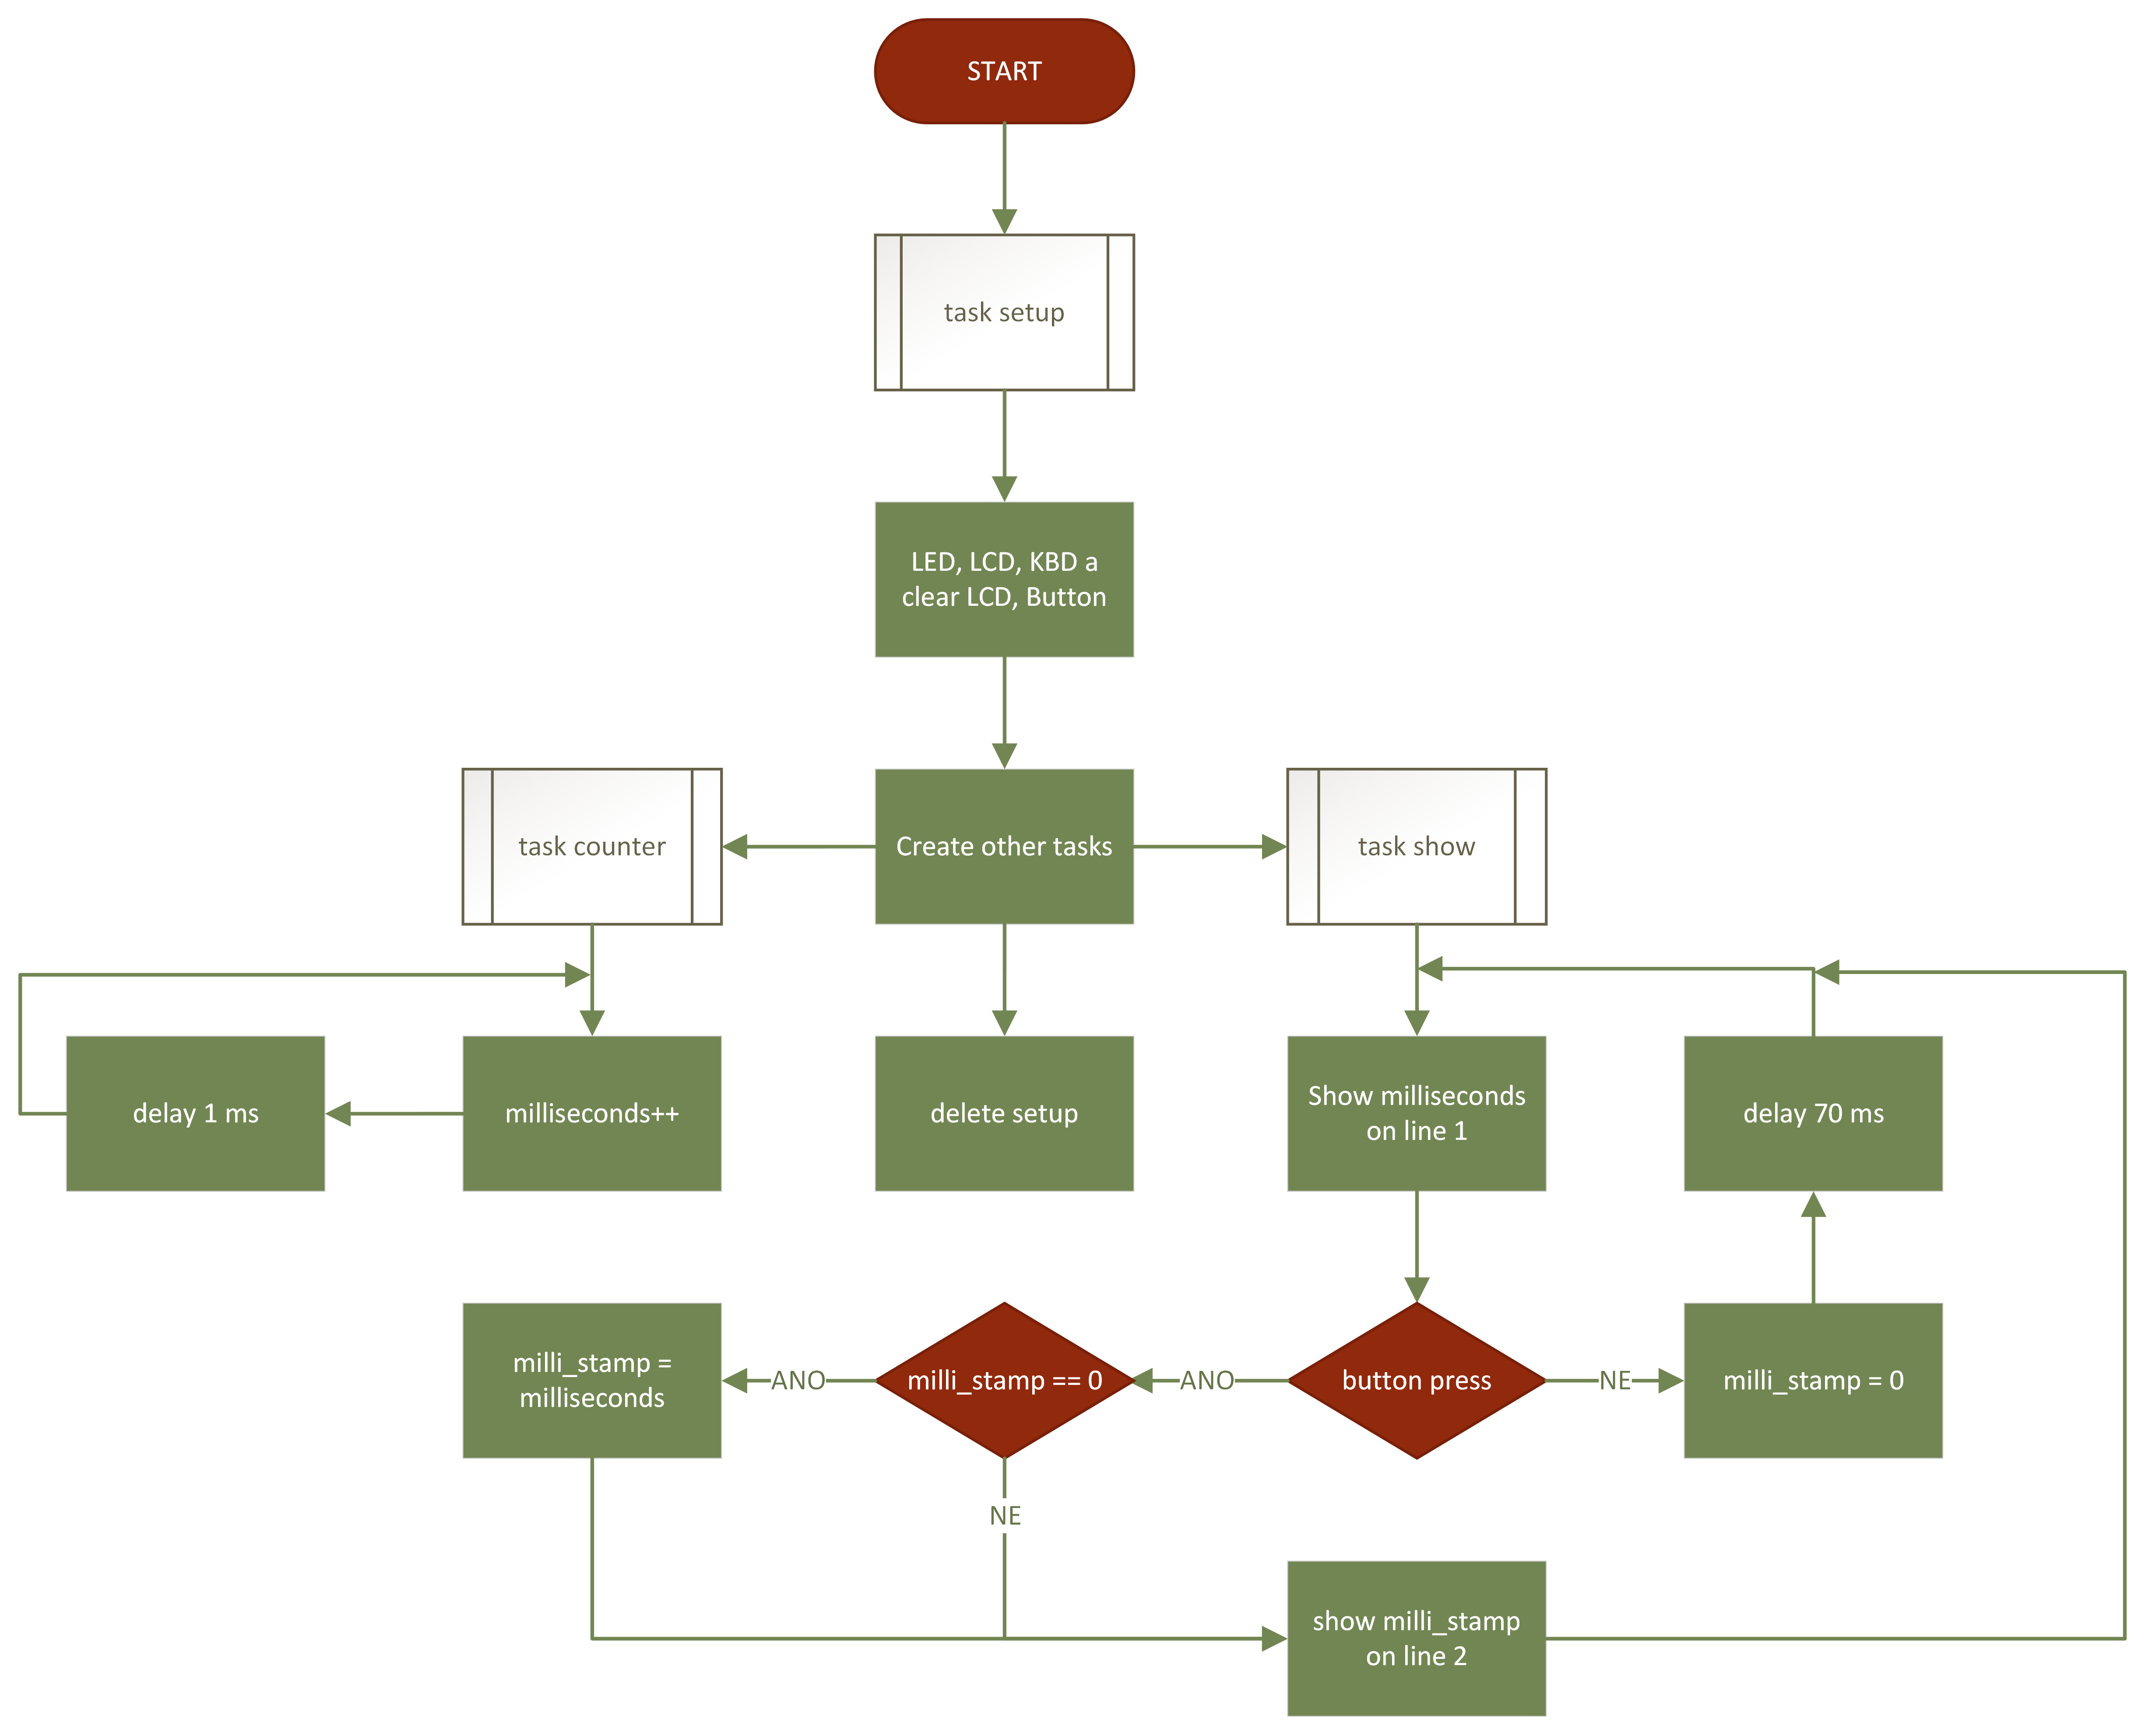
\includegraphics[scale=0.35]{flowchart.png}
    \caption{Vývojový diagram}
\end{figure}

\section{Řešení}

Vytvořil jsem dva tasky, kde: první počítá oběhnuté millisekundy, druhý task zobrazuje na LCD uběhnutý čas, a kontroluje zmáčknutí uživatelského tlačítka.

\subsection{Zdrojový kód}

\lstinputlisting[language=C]{stopky.c}

\section{Hodnocení}

Výsledek hodnotím kladně, podařilo se vyřešit zadání, v jednoduchém kódu.

\subsection{Úspěchy/neúspěchy}
Uspěšnost vidím ve splnění zadání, neúspěchy mohou být viděny v neoriginalitě řešení.

\subsection{Další rozšížení}
Jako dalši rozšíření vidím:
\begin{itemize}
    \item Přidání historie časů, a jejich ásledné prohlížení;
    \item Počítaní doby, jež uběhla mezi časy;
    \item Uživatelské tlačitkop bude v separátním tasku.
\end{itemize}

\end{document}
 